\documentclass{report}
\usepackage{graphicx} % Required for inserting images
\usepackage{braket}
\usepackage{float}
\usepackage{wrapfig}
\usepackage{amsmath}
\usepackage{amssymb}
\usepackage{braket}
\usepackage{cancel}
\usepackage{bbold}
\usepackage{upgreek}
\usepackage{tikz}
\usepackage{mathtools}
\DeclarePairedDelimiter{\ceil}{\lceil}{\rceil}


\title{Quantum Information}
\date{2025}
\author{Giuseppe Scordo}

\begin{document}

\maketitle

\chapter{Introduction}

Quantum information è un corso sulla teoria dell'informazione che si compone di 2 parti
\begin{itemize}
    \item 3 CFU di \textbf{Introduzine alla teoria classica}
    \item 3 CFU di \textbf{Introduzine alla teoria quantistica}
\end{itemize}
Cos'è la teoria dell'informazione?
\\Fino a che punto possiamo comprimere i dati? Qual'è il miglior tasso di trasmissione possibile?
\begin{itemize}
    \item \textbf{Teoria classica dell'informazione}
    \\ Ci chiediamo cosa sia l'informazione e come renderla affidabile su canali inaffidabili. Vediamo in breve cenni di teoria dell'infrmazione di Shannon:
    \begin{itemize}
        \item È possibile inviare informazione con probabilità di errore $\epsilon$, se il tasso di comunicazione è minore della capacità del canale
        \item Ogni segnale ha complessità intrinseca (\textit{entropia}) oltre al quale non può essere compreso
        \item Se l'entropia della sorgente è minore della capacità di canale, una comunicazione (asintoticamente) priva di errori può avvenire
    \end{itemize}
    \item  \textbf{Teoria dell'informazione quantistica}
    \\A differenza del caso precedente utilizziamo i qubit. Quello che fa davvero la differenza sono i \textit{termini di coerenza}, usando le matrici di densità. 
    Un'altra differenza è la presenza dell'\textbf{entanglement}.
    Studieremo come misurare l'entropia di uno stato quantistico (Entropia di Von Neumann).
\end{itemize}
Vedremo le seguenti misure: Capacità classica, quantistica e quantistica assistita (con entanglement)

\chapter{Informazione Classica}

\section{Canale binario simmetrico}
Trasmette messaggi bit a bit, ognuno dei quali potrebbe essere corrotto. 
$$f\rightarrow p(corr.) \Rightarrow 0 \leq f \leq 1$$
\begin{wrapfigure} {l}{0.5\textwidth}
    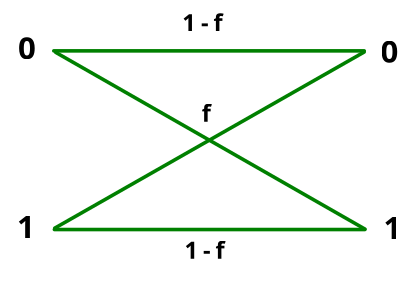
\includegraphics[width=1\linewidth]{Canale.png}

\end{wrapfigure}

Quindi con probabilità $f$ il bit verrà flippato.
\\Ipotizziamo $f = 0.1$. Allora con probabilità $0.9$ il bit sarà corretto.
\\ Possiamo risolvere gli errori utilizzando i \textbf{Codici di ripetizione}.
\\Scelgo un numero dispari (es. 3) e ripeto n volte il bit.
\\Se volessi inviare $0110$ con una codifica $R_3$ avremo 
$$0 \rightarrow 000 \hspace{1cm} 1 \rightarrow 111\hspace{1cm} 1 \rightarrow 111 \hspace{1cm}0 \rightarrow 000$$
Supponendo che nel canale ci siano stati errori avremmo che
$$010 \rightarrow 0 \hspace{1cm} 101 \rightarrow 1\hspace{1cm} 111 \rightarrow 1 \hspace{1cm}100 \rightarrow 0$$
Ovviamente questo metodo ha dei limiti perchè se l'errore non è distribuito bene non possiamo ricostruire correttamente l'informazione.
Usando $R_3$ l' errore diventa: $P[E_3] = \sum^{3}_{i=2} \binom{3}{i} f^i(1-f)^{3-i}=\binom{3}{2}f^2(1-f)+f^3 = 3f^2-2f^3=O(f^2)$
\\N.B. $0\leq f \leq1$, quindi $f^2 > f^3$.
\\Possiamo passare adesso da $f = \frac{1}{10}$ a $f = \frac{1}{100}$ con 5 ripetizioni. Notiamo che questa funzione vale per questo specifico canale senza perdita di bit. In $R_5$ abbiamo un tasso di pardita:
$$P[E_5 ]=\sum^{5}_{i=3} \binom{5}{i}f^i(1-f)^{5-i} = O(f^3)$$
Di conseguenza per un N generico di ripetizioni abbiano:
$$P[E_N]=\sum^{N}_{i=\frac{N+1}{2}} \binom{N}{i}f^i(1-f)^{N-i} = O(f^{\frac{N+1}{2}})$$
Notiamo che la crescita è lineare e che dovremmo usare troppo spazio per tassi d'errore tendenti allo zero.
\\Adesso supponiamo di avere $R_9$, dove $P[E_9]=O(f^6)$. Sfruttando una sua variante $R^2_3$, cioè codificando due volte in $R_3$, abbiamo che $$P[E_{R^2_3}]=\sum^{3}_{i=2}\binom{3}{i}P^i_{2R_3}(1-P_{2R_3})^{3-i} \approx O(f^4)$$
che è paggio, quindi paghiamo lo spazio con l'errore.
\\Introduciamo inoltre il \textbf{Tasso di trasmissione}, cioè il rapporto tra i bit che vogliamo inviare e quelli effettivamente codificati. Con una codifica $R_N$ il bitrate è di $\frac{1}{N}$, cioè molto scarso. 
\\Proviamo ad utilizzare i \textbf{Codici di Hamming(7,4)}.
\\Utilizziamo 7 bit per spedirne 4, dove $s_1,s_2,s_3,s_4$ sono i bit da inviare e $$t_1,t_2,t_3$$ sono di controllo.

\begin{figure} [H]
\centering
    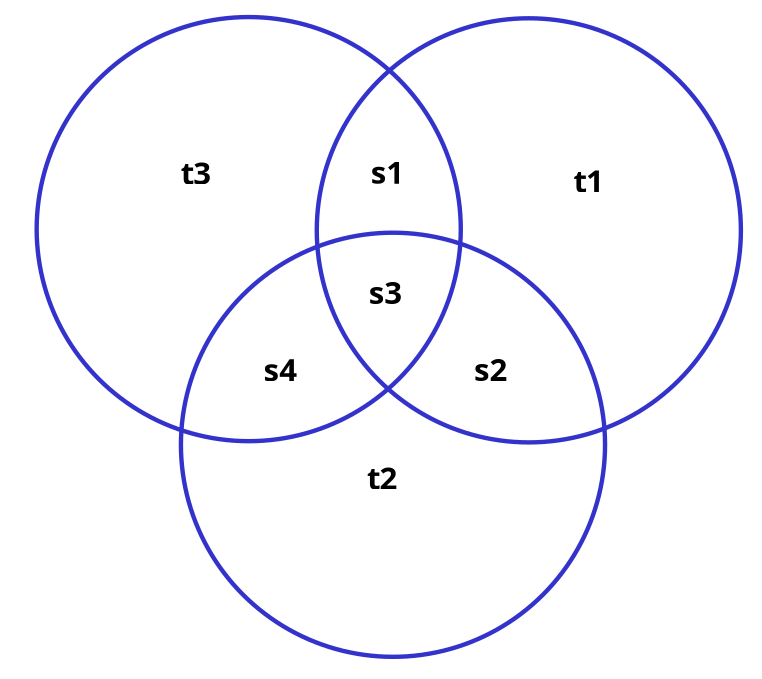
\includegraphics[width=0.5\linewidth]{hamming.png}

\end{figure}
scegliamo i controlli in modo che:
$$s_1+s_2+s_3+t_1=0 \mod2$$
$$s_2+s_3+s_4+t_2=0 \mod2$$
$$s_1+s_3+s_4+t_3=0 \mod2$$
Notiamo che il bitrate è di $\frac{4}{7}$, un po'meglio di $R$
\\Avendo un errore riscontreremo una \textit{Sindrome} che dovremo risolvere con il minor numero di modifiche possibili.
Con 2 errori però abbiamo già un problema. non possiamo più ricostruire l'informazione.
\\ Sia $E_H$ l'evento che i bit vengano inviati con errori. Allora la probabilità di averne 2 è:
$$P[E_H]=\sum^{7}_{i=2}\binom{7}{i}f^i(1-f)^{7-i}=O(f^2)$$
come per $R_3$ ma con un bitrate maggiore. 
\\Se vogliamo un tasso d'errore alto sembrerebbe che anche il bitrate debba esserlo. Shannon ci dice che possiamo avere un tasso d'errore basso e un bitrate consistentemente diverso da 0.

\section{Ripasso di probabilità}
Una \textbf{Variabile Aleatoria $X$} a valori in $A_x=(a_0,...,a_{n-1})$ associa ad ogni evento un numero
\\ \textbf{Assiomi della probabilità}:
\begin{description}
    \item[1.] Non negatività : dato $E,\hspace{0.4cm}P(E) \ge0$
    \item[2.] Additività : siano $A,B$ 2 V.A. indipendenti, $P[A\cup B]=P[A]+P[B]$
    \item[3.] Normalizzazione: sia $E$ l'evento certo, $P[E]=1 $
\end{description}
Da questi assiomi possiamo dimostrare tutti i teoremi sulle probabilità. Ad esempio dimostriamo l'evento impossibile.
$$P[E] = P[E\cup I]=P[E]+P[I]=1+P[I]\Rightarrow P[I] = P[E]-1 = 0$$
Da ora in poi useremo la notazione $P[A,B]=P[A\wedge B]$

Date 2 V.A. $X,Y$ con supporti $A_x,A_y$ valgono i seguenti teoremi:
\begin{itemize}
    \item Teorema delle probabilità totali: $P[X=x_i]=\sum_{y\in A_y}P[X=x_i \wedge Y = y_i]$
    \item Probabilità condizionata: $P[X|Y]=\frac{P[X\wedge Y]}{P[Y]}$
    \item Da cui segue: $P[X=x\wedge Y =y]=P[X=x|Y=y]P[Y=y]$
    \item Teorema di Bayes: $P[X|Y] = \frac{P[Y|X]P[X]}{P[Y]}$
\end{itemize}
 Daremo per scontate le ipotesi $H$ sotto la quale faremo i gli esempi, $P[X=x|H]$.
 
Il \textbf{Valore atteso} $E[X] = \sum_{x\in A_x}xP[X=x]$ rappresenta la nostra aspettativa dul valore di una V.A.
\\ \textbf{Proprietà}:
\begin{itemize}
    \item $E[X,Y] = E[X]+E[Y]$
    \\Dimostrazione: \\$E[X,Y]=\sum_x\sum_y(x+y)P(x\wedge y)= \sum_x \sum_y (xP(x\wedge y))+y(P(x\wedge y)) = \sum_x x \sum_y P(x,y) + \sum_y y \sum_x P(x,y) = \sum_x x P(x) + \sum_y y P(y) = E[X] +E[Y]$
    \item $E[cX] = cE[x]$ e $E[X+c] = E[X] + c$
    \item Supponendo $X,Y$ indipendenti $E[XY] = E[X]E[Y]$
    \\Dimostrazione: \\$E[XY] = \sum_{x,y} xyP(x\wedge y) = \sum_x\sum_y xy P(X)P(Y)=\sum_x\sum_y xP(x)yP(y) = \sum_x xP(X)\sum_y yP(Y) = E[X]E[Y]$
\end{itemize}

La \textbf{Varianza} $Var(X)=E[(X-E[X])^2]$ rappresenta la dispersione dei valori. Analogamente $ = E(X^2+E[X]^2-2E[X])=E[X^2]+E[X]^2-2E[X]E[X]=E[X^2]-E[X]^2$

\section{Informazione di Shannon}
\textbf{Informazioine di Shannon}: $h(x) = \log\frac{1}{P[X]}$
\\ \textbf{Formula dell'entropia}: $$H(X) = \sum_{x\in A_x}P[X]\log\frac{1}{P[X]} \hspace{0.5cm} 0\le H(X)\le \log \left| A_x \right| $$
L'entropia è massima quando l'incertezza è massima.
\\ \textbf{Ridondanza}: $1-\frac{H(X)}{\log \left| A_x \right|}$
\\ \textbf{Entropia congiunta}: $H(X,Y) = \sum_{x\in A_x,y\in A_y}P[X,Y] \log\frac{1}{P[X,Y]}$

\textbf{Proprietà}:
\begin{itemize}
    \item $H(X)\ge 0$
    \item $H(X)\le \log \left| A_x \right|$
    \item $H(X,Y) = H(X)+H(Y)$ se $X$ e $Y$ sono indipendenti
\end{itemize}

Dimostriamo le proprietà:
\\ Per la prima dimostrazione basta notare che $H(X) = \sum_x P(x)\log\frac{1}{P(x)}$ dove $0\le P(X) \le 1$ e di conseguenza anche $\log\frac{1}{P(X)}$ è non negativo 
\\ Per dimostrare la seconda abbiamo bisogno di alcune proprietà che vederemo dopo.
\\per dimostrare la terza introduciamo altre 2 proprietà:
\begin{itemize}
    \item $H(X|y = b) = \sum_xP[X|y=b]\log \frac{1}{P[X|y=b]}$
    \item $H(X|Y) = \sum_yP[Y]\sum_xP[X|Y]\log \frac{1}{P[X|Y]} = \sum_x\sum_yP[X,Y]\log\frac{1}{P(X|Y)}$
    \item Regola della catena per l'entropia: $H(X,Y) = H(X) + H(Y|X)$
\end{itemize}
Passando alla dimostrazione: \\$H(X,Y) = \sum_x\sum_yP[x,y]\log\frac{1}{P[x,y]}=\sum_x\sum_y P[x,y]\log\frac{1}{P[y|x]P[x]}=\sum_x\sum_yP[x,y](\log\frac{1}{P[y|x]})+\log\frac{1}{P[x]} = $$ \sum_{x,y} P[x,y]\log\frac{1}{P[y|x]}+\sum_{x,y}P[x,y]\log\frac{1}{P[x]}$ \\Adesso notiamo che $\sum_{x,y} P[x,y]\log\frac{1}{P[y|x]} = H(Y|X)$ e $\sum_{x,y}P[x,y]\log\frac{1}{P[x]} = H(x)$ per cui $H(X,Y) = H(Y|X)+H(X)$ da cui ovviamente per $X,Y$ indipendenti $H(X,Y) = H(Y)+H(X)$.

\textbf{Disuguaglianza di Jensen}
\\ Sia $f$ una funzione convessa 
\\(*$]a,b[ ,\forall x_1,x_2\in]a,b[,0\le\lambda\le1 \Rightarrow f(\lambda x_1+(1-\lambda)x_2)\le \lambda f(x_1)+(1-\lambda)f(x_2)$)
\\allora vale la seguente disuguaglianza: $$E[f(X)]\ge f(E[X])$$
Dimostriamola per induzione su $\left| A_x \right|$:
\\base: $\left| A_x \right| = 2 \hspace{0.5cm} x_1,x_2 \hspace{0.3cm} p_1,p_2=1-p_1$
$$E(f(X))=p_1f(x_1)+p_2(fx_2)=p_1(fx_1)+(1-p_1)f(x)\ge f(p_1x_1+(1-p_1)x_2)=f(E(X))$$
Ipotesi Induttiva: tesi vera per $\left| A_x \right| = k$, dimostriamo per $k+1$
$$E[f(X)] = \sum^{k+1}_{i=1}p_if(x_i)=p_{k+1}f(x_{k+1})+\sum^k_{i=1}p_if(x_i)$$
$$= p_{k+1}f(x_{k+1})+(1-p_{k+1})\sum^k_{i=1}\frac{p_i}{1-p_{k+1}}f(x_i)$$
Applicando Jensen:
$$\ge p_{k+1}f(x_{k+1})+(1-p_{k+1})f\left(\sum^k_{i=1}\frac{p_i}{1-p_{k+1}}x_i\right)$$
per la concavità di $f$:
$$\ge f\left(p_{k+1}x_{k+1}+(1-p_{k+1})\sum^k_{i=1}\frac{p_i}{1-p_{k+1}}x_i\right) = f\left(p_{k+1}x_{k+1}+\sum^k_{i=1}p_ix_i\right)$$
$$= f\left( \sum^{k+1}_{i=1}x_ip_i\right)=f(E[X])$$

\textbf{Entropia relativa (Divergenza di Kullback Leibler)}
$$D_{KL}(P||Q)=\sum_{x\in A_x}P(x)\log\frac{P(x)}{Q(x)}$$
\textbf{Disuguaglianza di Gibbs}
$$D_{KL}\ge 0$$
Dimostrazione: $-D_{KL}=-\sum_{x\in A_x}P(x)\log\frac{P(x)}{Q(x)}=\sum_{x}P(x)\log\frac{Q(x)}{P(x)}$
essendo il logaritmo una funzione concava applichiamo la disuguaglianza di Jensen
$$\le\log\sum_xP(X)\frac{Q(X)}{P(X)}=\log\sum_xQ(X)=\log1=0$$
Invertendo i sengni $-D_{KL}(P||Q)\le0 \Rightarrow D_{KL}(P||Q)\ge0$

Adesso possiamo finalmente dimostrare la proprietà per cui $H(X)\le\log\left|A_X\right|$
\\Sia $U$ la distribuzione uniforme
$$D_{KL}(P||U)=\sum_xP(x)\log\frac{P(x)}{U(x)}=\sum_xP(x)\left(\log P(x) +\log\frac{1}{U(x)}\right)$$
$$=\sum_xP(x)\log P(x)+\sum_xP(x)\log \frac{1}{U(x)}$$
Essendo $U$ la distribuzione uniforme $U(X)=\frac{1}{\left|A_x\right|}$

$$=-\sum_xP(x)\log \frac{1}{P(x)}+\sum_xP(x)\log \frac{1}{P(x)}=-H(X)+\sum_xP(x)\log{\left|A_x\right|} $$
$$=-H(X)+\log\left|A_x\right|$$
Applicando la disuguaglianza di Gibbs:
$$0\le -H(X)+\log\left|A_x\right| \Rightarrow H(X)\le\log\left|A_x\right|$$

\section{Mutua informazione}
La mutua informazione rappresenta la perdita di incertezza su $X$ noto $Y$
$$I(X;Y)=\sum_{x\in A_x, y\in A_y}P(X,Y)\log\frac{P(X,Y)}{P(X)P(Y)}$$
Dimostrazione: $I(X;Y)=\sum_{x,y}P(x,y)\log\frac{P(x,y)}{P(x)P(y)}=\sum_{x,y}P(x,y)\log\frac{P(x|y)P(y)}{P(x)P(y)}$
$=\sum_{x,y}P(x,y)(\log P(X|Y) + \log\frac{1}{P(X)})=\sum_{x,y}P(x,y)\log\frac{1}{P(x)}+\sum_{x,y}P(x,y)\log P(x|y )$
la prima parte per il teorema delle probabilità totali è semplicemente 
\\$= H(x)+\sum_{x,y}P(x,y)\log P(x|y)=H(X)-\sum_{x,y}P(x,y)\log\frac{1}{P(x|y)}$\\$=H(X)-H(X|Y)$

\textbf{Proprietà}
\begin{itemize}
    \item $I(X;X)=H(X)$
    \\Dimostrazione: $H(X)-H(X|X)=H(X)$
    \item  $I(X;Y)=I(Y;X)$
    \item $I(X;Y)\ge 0$
    \\Dimostrazione: $I(X;Y)=\sum_{x,y}P(x,y)\log\frac{P(x,y)}{P(x)P(y)}$ poniamo $\widehat{P}(x,y) = P(x,y)$ e $\widehat{Q}(x,y) = P(x)P(y)$ e applichiam la disuguaglianza di Gibbs.
\end{itemize}

\textit{Esercizio: Date 12 palline, sappiamo che 11 hanno lo stesso peso mentre una è più leggera o più pesente. Usando una bilancia puoi pesare contemporaneamente lo stesso numero di palle sul braccio destro e sinistro. Trova una strategia di pesata dimostrabilmente ottima.}
\\
Ci chiediamo adesso, come vincere al gioco del sottomarino? È una versione di battaglia navale con una sola casella da dover indovinare. La probabilità di indovinare è $P[Y]=\frac{1}{64}$ e qundi l'informazione di Shannon è $h(Y) = \log 64 = 6$ (\textit{che significa che guadagnamo 6 bit di informazione, infatti $2^6 = 64$}).
\\La probabilità di sbagliare al primo tentativo è $P[N] = \frac{63}{64}$ con $h(N)= \log \frac{64}{63} \approx 0,0224$ (\textit{guadagnamo pochissima informazione}). Notiamo che non essendoci reinserimento la probabilità di sbagliare al secondo tentativo sarà $P[N_2] = \frac{62}{63}$, al terzo $P[N_3]=\frac{61}{62}$ e così via.
\\Dopo 32 tentativi, cioè la metà, avremo che $\log(\frac{64}{\cancel{63}}\cdot \frac{\cancel{63}}{\cancel{62}} \dots \frac{\cancel{33}}{32}) = \log \frac{64}{32} = \log 2 = 1$. Abbiamo scoperto che dopo aver tentato 32 volte otteniamo solo un bit di informazione, cioè che il sottomarino non è nella prima metà delle caselle.

\section{Compressione}
Gli esempi visti giustificano l'idea che l'informazione di Shannon di un evento sia una misura naturale per l'informazione.
Risposte \textit{"improbabili"} portano maggiore informazione su una situazione. Se riuscissimo a comprimere una sorgente in un file a L-bit per simbolo allora l'informazione media contenuta  nella sorgente è al massimo  L-bit per simbolo.
\\Per enumerare tutti i possibili outcome $\left|A_x \right|$
\begin{itemize}
    \item Diamo un nome binario ad ogni risultato
    \item La dimensione di ogni nome è $\log \left|A_x \right|$
\end{itemize}
Definiamo \textbf{raw-bit content} di $X$ $$H_0 = \log \left|A_x \right| $$
Questo rappresenta un \textit{lower-bound} del numero di bit che permettono di rappresentare $X$. Data una codifica $c$
$$c(x)\hspace{0.5cm}  ,\forall x \hspace{0.25cm} c(x)\ge H_0(X)$$

\subsection{Compressione Lossy}
Potremmo decidere di perdere informazione per guadagnare in termini di dimensione. Immaginiamo di comprimere un file di testo, rimuovendo i caratteri non utilizzati spesso come "\{,\},\&,§,\#,@" possiamo avere più compressione. 
\\Indichiamo con $\delta$ la probabilità che non ci sia alcun simbolo per un outcome $x$.
\\Per una strategia con rischio $\delta$ consideriamo il più piccolo insieme $S_\delta$ t.c.
$$P(x\not \in S_\delta)\le \delta$$
minimo insieme $\delta$-sufficiente e minimo sottoinsieme $S_\delta$ di $A_x$ t.c.
$$P(x\in S_\delta)\ge 1- \delta$$

Definiamo \textbf{Essential bit content} (di $X$)
$$H_\delta(X)= \log \left|S_\delta\right|$$
Notiamo che se $\delta = 0$ corrisponde con il raw.
\\Vediamo un esempio:
\\Data una sequenza binaria di 4 bit, con \\$P[X=1]= 0,1 = p_1$ e $P[X=0]= 0,9 = p_0$ abbiamo
$$P[X=0000]=0,6561$$ $$P[X=\text{"ci sia un uno"}]=0,3036$$ $$P[X=\text{"ci siano due uno"}]=0,0486$$ $$P[X=\text{"ci siano tre uno"}]=0,0036$$ $$P[X=1111]=0,00014$$

Se consideriamo adesso $\delta = 0,01$ avremo 11 elementi in $S_\delta$, cioè tutti i casi con meno di tre uno.
$$H_\delta = \log \left|S_\delta \right| = 3,45$$
in questo caso, lavorando su numeri piccoli abbiamo ottenuto poco.
\\Possiamo normalizzare rispetto alla lunghezza $N$ di una qualsiasi stringa binaria
$$\frac{1}{N}H_\delta(x^N)$$
Per $N$  molto grandi la dipendenza da $\delta$ diventa poco significativa. Questo fenomeno è detto \textbf{Tipicalità}, cioè al crescere di $N$ la stringa più probabile aumenta il proprio peso e ci si avvicina al comportamento tipico.
\\Vale il \textbf{Teorema del Codice Sorgente} di Shannon:
\\Sia $X$ una v.a. con entropia $H$. Dato $\epsilon > 0$ e $0\le\delta\le 1$, allora esiste un intero $N_0$ t.c. per $N>N_0$ si ha $$\left| \frac{1}{N} H_\delta(X^N)-H \right| < \epsilon$$
\begin{description}
    \item[1.] $\frac{1}{N}H_\delta(X^N) < H +\epsilon$, è la tolleranza
    \item[2.] $\frac{1}{N}H_\delta(X^N) > H -\epsilon$, per $\epsilon$ tendenti a zero quasi non perdiamo molto
\end{description}

\subsection{Compressione non Lossy}
Utilizziamo \textbf{Codici simbolici}. Sia $X$ v.a. (su $A_x$) e $c:A_x\rightarrow\{0,1\}^*$ una codifica e definiamo inoltre $c(x)$ \textbf{codeword} e $l(x)$ \textbf{lunghezza}.
\newpage
Un buon codice dovrebbe comprimere quanto più possibile, e per fare ciò una prima possibilità è quella di utilizzare dei \textbf{Codici non univocamente Decodificabili.}
$$A_x = \{a,b,c,d \}, \hspace{0.5cm} P_x=\left\{ \frac{1}{2},\frac{1}{4},\frac{1}{8},\frac{1}{8} \right\}$$ 
$$c_1(a) = 0, \hspace{0.2cm} c_1(b) = 010, \hspace{0.2cm} c_1(c) = 01, \hspace{0.2cm} c_1(d) = 10$$
Il problema di questi codici è che è possibile determinare il risultato solo alla fine della lettura di tutto il messaggio. Se ad esempio avessimo $010$

\begin{center}
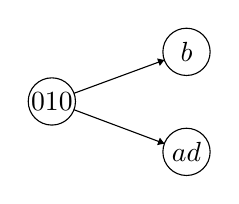
\begin{tikzpicture}[scale=0.1]
\tikzstyle{every node}+=[inner sep=0pt]
\draw [black] (13.7,-24.4) circle (3);
\draw (13.7,-24.4) node {$010$};
\draw [black] (30.8,-18.1) circle (3);
\draw (30.8,-18.1) node {$b$};
\draw [black] (30.8,-30.8) circle (3);
\draw (30.8,-30.8) node {$ad$};
\draw [black] (16.51,-25.45) -- (27.99,-29.75);
\fill [black] (27.99,-29.75) -- (27.42,-29) -- (27.07,-29.94);
\draw [black] (16.52,-23.36) -- (27.98,-19.14);
\fill [black] (27.98,-19.14) -- (27.06,-18.94) -- (27.41,-19.88);
\end{tikzpicture}
\end{center}
Per questa ragione passiamo ai \textbf{Codici univocamente decodificabili}
$$c^*(x) = c(x_1)c(x_2)\dots(c_t) \hspace{0.5cm} x = x_1\dots x_t$$
$$\forall x,y\in A_x \text{ se }x\neq y \Rightarrow c^*(x)\neq c^*(y)$$
Ad esempio definiamo la seconda codifica:
$$c_2(a) = 10, \hspace{0.2cm} c_2(b) = 00, \hspace{0.2cm} c_2(c) = 11, \hspace{0.2cm} c_2(d) = 110$$
Un modo per ottenere Codici univocamente decodificabili leggibili a runtime è quella di utilizzare dei \textbf{Codici prefix-free} (o \textit{istantanei})
$$c_3(a) = 0, \hspace{0.2cm} c_3(b) = 10, \hspace{0.2cm} c_3(c) = 110, \hspace{0.2cm} c_3(d) = 111$$

\begin{center}
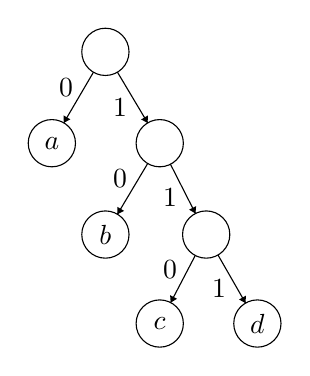
\begin{tikzpicture}[scale=0.1]
\tikzstyle{every node}+=[inner sep=0pt]
\draw [black] (39.8,-8.5) circle (3);
\draw [black] (33,-20.1) circle (3);
\draw (33,-20.1) node {$a$};
\draw [black] (46.7,-20.1) circle (3);
\draw [black] (39.8,-31.7) circle (3);
\draw (39.8,-31.7) node {$b$};
\draw [black] (52.6,-31.7) circle (3);
\draw [black] (46.7,-43) circle (3);
\draw (46.7,-43) node {$c$};
\draw [black] (59.1,-43) circle (3);
\draw (59.1,-43) node {$d$};
\draw [black] (38.28,-11.09) -- (34.52,-17.51);
\fill [black] (34.52,-17.51) -- (35.35,-17.07) -- (34.49,-16.57);
\draw (35.75,-13.05) node [left] {$0$};
\draw [black] (41.33,-11.08) -- (45.17,-17.52);
\fill [black] (45.17,-17.52) -- (45.19,-16.58) -- (44.33,-17.09);
\draw (42.61,-15.56) node [left] {$1$};
\draw [black] (45.17,-22.68) -- (41.33,-29.12);
\fill [black] (41.33,-29.12) -- (42.17,-28.69) -- (41.31,-28.18);
\draw (42.61,-24.64) node [left] {$0$};
\draw [black] (48.06,-22.77) -- (51.24,-29.03);
\fill [black] (51.24,-29.03) -- (51.32,-28.09) -- (50.43,-28.54);
\draw (48.96,-27.02) node [left] {$1$};
\draw [black] (51.21,-34.36) -- (48.09,-40.34);
\fill [black] (48.09,-40.34) -- (48.9,-39.86) -- (48.02,-39.4);
\draw (48.97,-36.2) node [left] {$0$};
\draw [black] (54.1,-34.3) -- (57.6,-40.4);
\fill [black] (57.6,-40.4) -- (57.64,-39.46) -- (56.77,-39.96);
\draw (55.19,-38.58) node [left] {$1$};
\end{tikzpicture}
\end{center}
Possiamo chiederci quindi qual'è la \textbf{lunghezza attesa} di un codice in una codifica prefix-free?
$$L(c,X)=\sum_{x\in A_x}P[x]l(x)$$
Nel caso della nostra codifica
$$L(c_3,X)=\frac{1}{2}\cdot1+\frac{1}{4}\cdot2+\frac{1}{8}\cdot3+\frac{1}{8}\cdot3= \frac{7}{4}=1,75$$
E adesso notiamo che:
$$H(X)=\sum_{x\in A_x}P(x)\log\frac{1}{P(x)}=\frac{1}{2}\cdot\log2+\frac{1}{4}\cdot\log4+\frac{1}{4}\cdot\log8=\frac{7}{4}$$
\textbf{Disuguaglianza di Kraft} (\textit{per codici prefix-free su alfabeti binari})
\\$X$ v.a. su $A_x$, sia $c$ una codifica prefix-free in $\{0,1\}^*$
$$\sum^{|A_x|}_{i=1}2^{-li}\le1$$
Dimostrazione: sia \textit{lmax}, la codeword di lunghezza massima. Il numero delle foglie sarà al massimo $2^{\textit{lmax}}$, se ci sono potature il numero totale di foglie sarà: 
$$\sum^{|A_x|}_{i=1}2^{\textit{lmax-li}}\le2^{\textit{lmax}}$$
$$\Rightarrow 2^{lmax}\sum^{|A_x|}_{i=1}2^{\textit{-li}}\le2^{lmax} \Longrightarrow\sum^{|A_x|}_{i=1}2^{\textit{-li}}\le1$$
Se una codifica soffisfa la disuguaglianza di Kraft $\Rightarrow$ è prefix-free
\subsection{Codici ottimi}
Minimizziamo $L(c,X)$ con lunghezze che soddisfano la disuguaglianza di Kraft. La lunghezza attesa di ogni codice binario è sempre $\ge H(X)$
$$L(c,X)\ge H(X)$$
Dimostrazione: $$L(c,X)-H(X)= \sum_i p_i l_i- \sum_i p_i\log \frac{1}{p_i}$$
Definiamo $g_i = \frac{2^{-li}}{z}$, e $z = \sum_j 2^{-lj}$. Avremo che $l_i = \log2^{li} = \log\frac{1}{g_iz}= \log\frac{1}{g_i}+ \log\frac{1}{z}$. Per cui:
$$=\sum_i p_i (\log\frac{1}{g_i}+\log\frac{1}{z}) - \sum_i p_i \log\frac{1}{p_i} =\sum_i p_i \log\frac{1}{g_i} +\sum_ip_i\log\frac{1}{z} + \sum_i p_i \log p_i$$
$$= \log \frac{1}{z}+ \sum_i p_i (\log\frac{1}{g_i}+\log p_i) = \log\frac{1}{z} + \sum_i p_i\log\frac{p_i}{g_i} $$$$= \log\frac{1}{z} + D_{KL}(p,g)\ge \log\frac{1}{z}\ge0$$

Quindi $L(c,X)-H(X)\ge0\Rightarrow L(c,X)\ge H(X)$
\\Supponiamo $l_i = \log \frac{1}{p_i}$, soddisfa la disuguaglianza di Kraft?
$$\sum_i 2^{-li}=\sum_i2^{-\log\frac{1}{p_i}}= \sum_i2^{\log p_i}=\sum_i p_i = 1$$
È sicuramente un intero? NO, quindi $l_i = \ceil[\big]{\log\frac{1}{p_i}} $
\medskip
\\ \textbf{Codice sorgente per codici simbolici}
$$H(X)\le L(c,X)\le H(X)+1$$
\\ \textbf{Dim.}
$$L(c,X)= \sum_ip_il_i=\sum_i p_i\ceil{\log \frac{1}{p_i}} \le \sum_ip_i(\log\frac{1}{p_i} + 1)$$
$$ = \sum_ip_i\log \frac{1}{p_i}+\sum_ip_i = H(X)+1 $$

Spesso la distribuzione di probabilità che usiamo non è quella reale ma approssimata ad una distribuzione $q_x$
\medskip
\\ \textbf{Teorema (Codici sbagliati)}
$$H(X)+D_{KL}(p||q)\le L(c,X)\le H(X)+D_{KL}(p||q)+1$$
\\ \textbf{Dim.}
$$
    L(c,X)=\sum_x p(x)l(x) = \sum_x p(x) \ceil{\frac{1}{q(x)}} \le \sum_x p(x)(\log\left(\frac{1}{q(x)}\right)+1)
$$
$$
    = \sum_x p(x)(\log\left(\frac{p(x)}{q(x)}\cdot\frac{1}{p(x)}\right)+1)= \sum_x p(x)\log\frac{p(x)}{q(x)}+\sum_x p(x)\log\frac{1}{p(x)}+\sum_x p(x)
$$
$$ = D_{KL}+H(x) + 1$$

\subsection{Codici di Huffman}
Usa un approccio bottoma up, collegando dal basso verso l'alto i caratteri con le probabilità più basse. I nodi avranno come label la somma delle probabilità dei nodi sottostanti, fino alla radie che ovviamente avrà come valore 1, essendo una distribuzione di probabilità.
\medskip
\\$A_x = \{a,b,c,d,e\} \hspace{0.5cm} P_x = \left\{ \frac{1}{4}, \frac{1}{4}, \frac{1}{5}, \frac{15}{100}, \frac{15}{100} \right \}$


\begin{center}
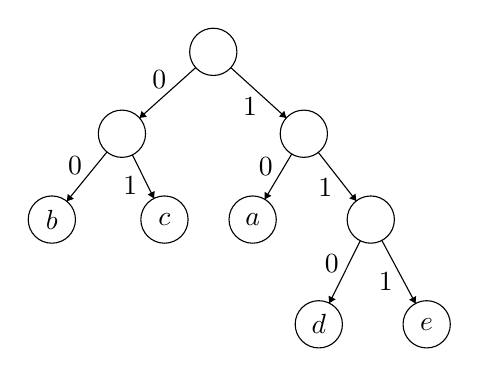
\begin{tikzpicture}[scale=0.1]
\tikzstyle{every node}+=[inner sep=0pt]
\draw [black] (40.2,-9.3) circle (3);
\draw [black] (28.6,-19.7) circle (3);
\draw [black] (51.7,-19.7) circle (3);
\draw [black] (19.7,-30.6) circle (3);
\draw (19.7,-30.6) node {$b$};
\draw [black] (34,-30.6) circle (3);
\draw (34,-30.6) node {$c$};
\draw [black] (45.2,-30.6) circle (3);
\draw (45.2,-30.6) node {$a$};
\draw [black] (60.2,-30.6) circle (3);
\draw [black] (53.6,-43.9) circle (3);
\draw (53.6,-43.9) node {$d$};
\draw [black] (67.3,-43.9) circle (3);
\draw (67.3,-43.9) node {$e$};
\draw [black] (37.97,-11.3) -- (30.83,-17.7);
\fill [black] (30.83,-17.7) -- (31.76,-17.54) -- (31.1,-16.79);
\draw (33.33,-14.01) node [above] {$0$};
\draw [black] (26.7,-22.02) -- (21.6,-28.28);
\fill [black] (21.6,-28.28) -- (22.49,-27.97) -- (21.72,-27.34);
\draw (23.59,-23.72) node [left] {$0$};
\draw [black] (29.93,-22.39) -- (32.67,-27.91);
\fill [black] (32.67,-27.91) -- (32.76,-26.97) -- (31.87,-27.42);
\draw (30.6,-26.25) node [left] {$1$};
\draw [black] (42.43,-11.31) -- (49.47,-17.69);
\fill [black] (49.47,-17.69) -- (49.22,-16.78) -- (48.55,-17.52);
\draw (44.88,-14.99) node [below] {$1$};
\draw [black] (50.16,-22.28) -- (46.74,-28.02);
\fill [black] (46.74,-28.02) -- (47.58,-27.59) -- (46.72,-27.08);
\draw (47.81,-23.89) node [left] {$0$};
\draw [black] (53.54,-22.07) -- (58.36,-28.23);
\fill [black] (58.36,-28.23) -- (58.26,-27.3) -- (57.47,-27.91);
\draw (55.38,-26.56) node [left] {$1$};
\draw [black] (58.87,-33.29) -- (54.93,-41.21);
\fill [black] (54.93,-41.21) -- (55.74,-40.72) -- (54.84,-40.27);
\draw (56.2,-36.15) node [left] {$0$};
\draw [black] (61.61,-33.25) -- (65.89,-41.25);
\fill [black] (65.89,-41.25) -- (65.95,-40.31) -- (65.07,-40.78);
\draw (63.07,-38.42) node [left] {$1$};
\end{tikzpicture}
\end{center}

$$
    H(X)=\frac{1}{2}\log4+\frac{1}{5} \log5+\frac{3}{10}\log\frac{3}{20} \approx2,28
$$
$$
    L(c,X) = \frac{1}{2}+\frac{2}{5}+\frac{9}{10} = 2,3
$$
Abbiamo verificato tramite un esercizio che un approccio top-down, ad esempio cercando di aver ogni sotto nodo con la metà della probabilità, non risulta essere molto buono.

\subsection{Comunicazione su canali inaffidabili}
Per il momento introduciamo solo due misure: $X$ segnale inviato e $Y$ segnale ricevuto. Il problema che ci interessa risolvere è quello della mutua informazione $I(X,Y)=H(X)-H(X|Y)$.
\\Esercizio.

\begin{table}[H]
    \centering
    \renewcommand{\arraystretch}{1.5} % <- AUMENTA L'ALTEZZA DELLE RIGHE
    \begin{tabular}{|c|c|c|c|c|}
        \hline
        $P(x,y)$ & $x=1$ & $x=2$ & $x=3$ & $x=4$ \\
        \hline
        $y=1$ & $\frac{1}{8}$ & $\frac{1}{16}$ & $\frac{1}{32}$ & $\frac{1}{32}$ \\
        \hline
        $y=2$ & $\frac{1}{16}$ & $\frac{1}{8}$ & $\frac{1}{32}$ & $\frac{1}{32}$ \\
        \hline
        $y=3$ & $\frac{1}{16}$ & $\frac{1}{16}$ & $\frac{1}{16}$ & $\frac{1}{16}$ \\
        \hline
        $y=4$ & $\frac{1}{4}$ & $0$ & $0$ & $0$ \\
        \hline
    \end{tabular}
    \label{tab:my_label}
\end{table}

$$p(x=1) = \frac{1}{8} + \frac{1}{16} + \frac{1}{16} + \frac{1}{4} = \frac{1}{2}$$
$$p(x=2) = \frac{1}{16} + \frac{1}{8} + \frac{1}{16} = \frac{1}{4}$$
$$p(x=3) = \frac{1}{32} + \frac{1}{32} + \frac{1}{16} = \frac{1}{8}$$
$$p(x=4) = \frac{1}{32} + \frac{1}{32} + \frac{1}{16} = \frac{1}{8}$$

$$ H(X) = \sum_xp(x) \log\frac{1}{p(x)} = \frac{7}{4}$$

$$H(Y) = \sum_y p(y)\log \frac{1}{p(y)} = 2$$

$$H(X,Y) = \sum_{x,y}p(x,y)\log\frac{1}{p(x,y)}= H(X)+H(Y|X) = H(Y)+H(X|Y) = \frac{27}{8}$$

$$ H(Y|X)= \frac{27}{8}-\frac{7}{4}$$

$$H(X|Y) = H(X,Y)-H(Y) = \frac{11}{8}$$

$$I(X,Y)=H(X)-H(X,Y)= \frac{3}{8}$$













%% Informazione quantistica


\chapter{Informazione Quantistica}
\section{Algebra Lineare}
Consideriamo lo \textbf{spazio di Hilbert} $\mathbb{C}^d$ dei vettori colonna sui numeri complessi:
$$
v =
\begin{pmatrix}
  v_1 \\
  v_2 \\
  \vdots \\
  v_d
\end{pmatrix},
\hspace{0.3cm} v_i \in \mathbb{C}
$$
Dotato del prodotto scalare $\braket{v|w} = \sum^{d-1}_{i=0}\bar{v_i}w_i$.
Se $\mathcal{H}$ è uno spazio di Hilbert arbitrario con $\dim(\mathcal{H} = d)$ finita, posso scegliere una \textit{Base ortonormale} $\left\{ \ket{e_i} \right\}^d_{i=1}$ di $\mathcal{H}$, cioè t.c
$$\braket{e_i|e_j} 
\begin{cases}
 \hspace{0.2cm}1 \hspace{0.8cm} i=j \\
 \hspace{0.2cm}0 \hspace{0.8cm} i\neq j
\end{cases}
$$
Indichiamo i vettori di $\mathcal{H}$ con il simbolo $\ket{\Psi}$ e $\bra{\psi}$ per il suo duale,
\\ \textbf{Base Ortonormale standard} di $\mathcal{H} = \mathbb{C}^d$
$$
\ket{0}=
\begin{pmatrix}
    1 \\
    0 \\
    \vdots \\
    0
\end{pmatrix}, 
\ket{1}=
\begin{pmatrix}
    0 \\
    1 \\
    \vdots \\
    0
\end{pmatrix}, \dots,
\ket{d-1}=
\begin{pmatrix}
    0 \\
    0 \\
    \vdots \\
    0
\end{pmatrix}
$$

Se $\ket{\Psi} = 
\begin{pmatrix}
    \psi_1 \\
    \psi_2 \\
    \vdots \\
    \psi_{d-1}
\end{pmatrix}
$
 allora $\ket{\Psi} = \sum^{d-1}_{i=0}\psi_i \ket{i}$ e il suo duale è $$\bra{\Psi} = \left(\bar{\psi_0},\bar{\psi_1},\dots,\bar{\psi}_{d-1} \right)$$

 Il prodotto scalare soddisfa la \textbf{Disequazione di Schwartz}:
 $$\forall \ket{\Phi},\ket{\Psi} \in \mathcal{H} = \mathbb{C}^d, \hspace{0.2cm} \left|\braket{\Phi|\Psi} \right|^2 \le \braket{\Phi|\Phi} \cdot \braket{\Psi|\Psi}$$
 E vale solo se $\ket{\Phi} = k\ket{\Psi}, \exists k \in\mathbb{C}$.
 \\La norma indotta del prodotto scalare è $\left| \left| \Psi\right| \right| = \sqrt{\braket{\Psi|\Psi}}$, per cui possiamo riscrivere il lemma di Schwartz come:
 $$\braket{\Phi|\Psi} = \left| \left|\Phi \right| \right| \cdot \left| \left|\Psi \right| \right|$$
 \subsection{Mappe lineari e matrici}
Utilizziamo funzioni lineari $f$, con le seguenti proprietà
\begin{description}
    \item[1.] $f(\lambda x) = \lambda f(x)$,
    \item[2.] $f(x+y) = f(x) + f(y)$ 
\end{description}
Dati $\mathcal{H}= \mathbb{C}^d, \mathcal{K} = \mathbb{C}^e$ spazi di Hilbert, $\textit{lin}(\mathcal{H},\mathcal{K})$ è l'insieme delle mappe lineari da $\mathcal{H}$ a $\mathcal{K}$. Se fissiamo una base per $\mathcal{H}$ e una base per $\mathcal{K}$ allora ogni mappa di $\textit{lin}(\mathcal{H},\mathcal{K})$ può essere scritta come una matrice $d\times e$
$$\textit{lin}(\mathcal{H},\mathcal{H}) = \textit{lin}(\mathcal{H}) \hspace{0.5cm} \mathbb{1} \text{ op. identità}$$
La \textbf{Traccia} di $M \in \textit{lin}(\mathcal{H})$ si calcola scegliendo una base $\Sigma$ di $\mathcal{H}$ e sommando gli elementi della diagonale principale.
$$\text{tr}[M] = \sum_{i \in \Sigma} \braket{i|M|i}$$
La traccia  è un invariante  per cambiamenti di base e soddisfa 
$$\text{tr}[MN] = \text{tr}[NM],\hspace{0.4cm} \forall M\in \textit{lin}(\mathcal{H,K}),N\in \textit{lin}(\mathcal{K,H})$$
Se $M\in \textit{lin}(\mathcal{H})$ e $N = \ket{\Psi}\bra{\Psi}$ per $\ket{\Psi}\in \mathcal{H}$ allora 
$\text{tr}[MN]=\braket{\Psi|M|\Psi}$
\\Se $M\in \textit{lin}(\mathcal{H})$ e $\exists\ket{\Psi}\in \mathcal{H}$ non nullo e $n \in \mathbb{C}$ t.c $M \ket{\Psi} = \lambda \ket{\Psi}$ allora $\ket{\Psi}$ è un \textbf{Autovettore} di $M$ con \textbf{Autovalore} $\lambda$.
\\Se $M\in \textit{lin}(\mathcal{H}_1,\mathcal{H}_2)$, dove $\mathcal{H}_1$ ha base $\Sigma_1$ e  $\mathcal{H}_2$ ha base $\Sigma_2$ allora 
$$M = \sum_{i \in \Sigma_1}\sum_{j \in \Sigma_2} M_{ij} \ket{i}\bra{j}\hspace{0.2cm} \text{e} \hspace{0.2cm} M_{ij} = \braket{i|M|j}$$
Sia  $M\in \textit{lin}(\mathcal{H}_1,\mathcal{H}_2)$, l'\textbf{Operatrore aggiuto} di $M$ è il \textit{"dagger"} di $M$
$$M^\dagger = \overline{M}^T$$
ed è tale che $$\braket{\Psi|M|\Phi} = \overline{\braket{\Phi|M^\dagger|\Psi}}$$
Ed inoltre $M^\dagger\in \textit{lin}(\mathcal{H}_2,\mathcal{H}_1)$ e $M^\dagger = \sum_{i,j} \overline{M_{ij}} \cdot\ket{j}\bra{i}$
\newpage
$M\in \textit{lin}(\mathcal{H})$ è \textbf{Hermitiano} (o autoaggiunto) se $M = M^\dagger$, cioè significa che $M$ ha elementi diagonali $M_{ii}$ reali e $M_{ij} = \overline{M_{ij}}$ per $i\neq j$.

$$\begin{pmatrix}
    1 & 1+i \\
    1-i & 0\\
\end{pmatrix}$$
Le matrici Hermitiane hanno autovalori reali e ammettono una base di autovettori.
\medskip
\\ \textbf{Teorema Spettrale}
\\Sia $M\in \textit{lin}(\mathcal{H})$ Hermitiana e $\dim (\mathcal{H} = d)$,\\ allora 
$\exists \lambda_1\ge\lambda_2\ge\dots\ge \lambda_d \in \mathbb{R}$ e una base $\left\{\ket{\Psi}\right\} ^d_{i=1} $ t.c.
$$M = \sum^d_{i=1}\lambda_i \ket{\Psi_i}\bra{\Psi_i}\hspace{0.4cm} \text{e\hspace{0.4cm} $\left\{ \lambda\right\} ^d_{i=1} $ si chiama \textbf{Spettro di M}}$$

Questo teorema ci dice che una matrice hermitiana può essere diagonalizzata usando matrici unitarie e la matrice diagonale ha elementi reali.
\medskip
\\OSS: lo spettro è univocamente è univocamente determinato da $M$ ma gli autovalori potrebbero essere non unici se lo spettro è degenere.
\\esempio: $\mathbb{1} = \sum^d_{i=1}\ket{\Psi_i}\bra{\Psi_i}, \hspace{0.2cm} \forall \left\{ \ket{\Psi_i}\right\} ^d_{i=1}$ 

\medskip
Se $M$ è Hermitiano  (o unitario) e $f$ è una funzione a una variabile, allora
$$f(M) = \sum^d_{i=1} f(\lambda_i)\ket{\Psi_i} \bra{\Psi_i}$$
Ossia: bisogna che $f$ sia ben definita sullo spettro.

\medskip
\textbf{Operatori Positivi}
\\$P \in \textit{lin}(\mathcal{H})$ è \textbf{Semidefinito positivo} (\textit{PSD}) oppure solo \textit{positivo} se
$$\forall \ket{\Psi} \in \mathcal{H}, \braket{\Psi|P|\Psi} \ge 0$$
\textbf{PSD($\mathcal{H})$} è l'insieme degli operatori $P\ge 0$ su $\mathcal{H}$
\medskip

$P \in \textit{lin}(\mathcal{H})$ è \textbf{Definitivo positivo} (\textit{PD}) $P > 0$ se $\forall \braket{\Psi|P| \Psi} > 0$

\medskip
\textit{PD($\mathcal{H}$)} è l'insieme degli operatori $P > 0$ su $\mathcal{H}$

\medskip 
\textbf{Lemma (caratterizzazione degli operatori PSD):} $P \in \textit{lin}(\mathcal{H})$ equivale a dire:
\begin{description}
    \item[a.] $P$ è \textit{PSD}, $\braket{\Psi|P|\Psi} \ge 0 \hspace{0.4cm} \forall\ket{\Psi}\in\mathcal{H}$ 
    \item[b.] $P$ è Hermitiano e i suoi autovalori sono non negativi
    \item[c.] $\exists M \in \textit{lin}(\mathcal{H,K}):P=M^\dagger M \hspace{0.3cm} \exists \mathcal{K}$ sp. di Hilbert
    \item[d.] $\forall Q \in PSD(\mathcal{H}), \text{tr}[PQ] \ge 0$
\end{description}
\textbf{Corollario:} Se $P \in PSD(\mathcal{H}), M \in \textit{lin}(\mathcal{H,K})$ allora $MPM^\dagger \in PSD(\mathcal{K})$
\\$P\le Q \Leftrightarrow Q-P \ge 0$, Questa nozione induce un ordinamento

\newpage
\textbf{Matrici Unitarie e Isometrie}
\\$V \in \textit{lin}(\mathcal{H,K})$ è \textbf{Isometria} se $V^\dagger V = \mathbb{1}$ (solo se $\dim(\mathcal{H}) \le\dim(\mathcal{K})$)
\\$V\in \textit{lin}(\mathcal{H})$ è \textbf{Unitaria} se $U^\dagger U = UU^\dagger = \mathbb{1}$
\\Deiniamo $U(\mathcal{H})$ l'insieme delle matrici unitarie su $\mathcal{H}$.

\medskip
$\textit{Isom}(\mathcal{H,K})$ insieme delle matrici isometrie da $\mathcal{H}$ a $\mathcal{K}$

\medskip
$P \in \textit{lin}(\mathcal{H})$ è una \textbf{Proiezione} se $P^2 = P$ e $P$ è Hermitiana.
\\Sia $\left\{\ket{e_i} \right\}^d_{i=1}$ base per l'immagine di una proiezione $P$, allora $P = \sum^d_{i=1}\ket{e_i}\bra{e_i}$

\medskip
Supponiamo $M$ Hermitiana, allora $M = \sum^d_{i=1} \lambda_i \ket{\Psi_i}\bra{\Psi_i}$

\medskip
I proiettori sono $P_\lambda = \sum_{i=\lambda} \ket{\Psi_i}\bra{\Psi_i}$

\medskip
Se $\Lambda =$ insieme degli autovalori \underline{distinti}, $M = \sum_{\lambda\in \Lambda} \lambda P_\lambda$ 

\medskip
In generale $M\in\textit{lin}(\mathcal{H,K})$ , $M = \sum^r_{i=1} s_i\ket{e_i}\bra{f_i}$ con $s_i\ge0$ autovalori, $r = \textit{rank}(M)$ e $e_i,f_i$ basi di $\mathcal{H}$ e $\mathcal{K}$.

\subsection{Prodotti tensoriali}
Def. $\mathcal{H,K}$ spazi di Hilbert. Il loro \textbf{Prodotto tensoriale $\mathcal{H} \otimes \mathcal{K}$} è lo spazio di Hilbert che contiene tutte le combinazioni lineari di vettori della forma $v \otimes u, \hspace{0.2cm} v\in\mathcal{H}, w \in \mathcal{K}$
\begin{itemize}
    \item $(\alpha v) \otimes (\beta w) = \alpha\beta \cdot v\otimes w, \hspace{0.2cm} \forall\alpha,\beta \in \mathbb{C}$
    \item $(v_1 + v_2) \otimes w = v_1 \otimes w + v_2 \otimes w$
    \item $v + (w_1 \otimes w_2) = v \otimes w_1 + v \otimes w_2$
\end{itemize}
Il prodotto scalare è definito da
$$\braket{v_1 \otimes w_2 |v_2 \otimes w_2} = \braket{v_1|v_2} \otimes\braket{w_1|w_2}$$
Base di $\mathcal{H} \otimes \mathcal{K} \hspace{0.5cm} \left\{ \ket{i} \otimes\ket{j} \right\}, \ket{i}\in B_\mathcal{H}, \ket{j} \in B_\mathcal{K}$

\medskip
$\ket{\Phi}\ket{\Psi} = \ket{\Phi\Psi} = \ket{\Phi} \otimes \ket{\Psi}$

\medskip
$\ket{\Phi} ^{\otimes n} = \ket{\Phi} \otimes \dots \otimes \ket{\Phi} \hspace{0.5cm} \mathcal{H}^{\otimes n} = \mathcal{H} \otimes\dots\otimes\mathcal{H}$

\medskip
Se $M \in \textit{lin}(\mathcal{H}_1,\mathcal{H}_2)$ e $N \in \textit{lin}(\mathcal{K}_1,\mathcal{K}_2)$ allora
$$M\otimes N : \mathcal{H}_1 \otimes \mathcal{K}_1 \longrightarrow \mathcal{H}_2 \otimes \mathcal{K}_2 $$
$$(M \otimes N) (\ket{ \Phi} \otimes \ket{\Psi}) = M\ket{\Phi} \otimes N \ket{\Psi}$$
$$\textit{lin}(\mathcal{H}_1\otimes\mathcal{K}_1,\mathcal{H}_2\otimes\mathcal{K}_2) = \textit{lin}(\mathcal{H}_1,\mathcal{H}_2) \otimes \textit{lin}(\mathcal{K}_1,\mathcal{K}_2)$$
$$M = \sum_{i,j}M_{ij}\ket{i}\bra{j}, \quad N = \sum_{k,l} N_{kl} \ket{k}\bra{l}$$
$$M \otimes N = \sum_{i,j,k,l} M_{ij} N_{kl}\ket{i}\bra{j} \otimes \ket{k}\bra{l} = \sum_{i,j,k,l} M_{ij} N_{kl}\ket{ik}\bra{jl}$$

\newpage
\textbf{Lemma}
\begin{description}
    \item[a.] $P \in \textit{PSD}(\mathcal{H}), Q \in \textit{PSD}(\mathcal{K}) \Rightarrow P \otimes Q \in \textit{PSD}(\mathcal{H}\otimes\mathcal{K})$
    \item[b.] $\forall M \in \textit{lin}(\mathcal{H}), N \in \textit{lin}(\mathcal{K}), \text{ tr}[M\otimes N] = \text{tr}[M]\text{tr}[N]$
    \item[c.] $\forall M \in \textit{lin}(\mathcal{H}), N \in \textit{lin}(\mathcal{K}), \text{ rank}(M\otimes N) = \text{rank}(M)\text{rank}(N)$
    \item[d.] $\ket{\Phi}\otimes z = z\ket{\Phi}, z \in \mathbb{C} \hspace{1cm}\mathcal{H} \otimes \mathbb{C}= \mathcal{H}$
    \item[e.] $M\otimes \ket{\Psi}: \mathcal{H} \longrightarrow \mathcal{H} \otimes \mathcal{K} \hspace{0.8cm} (M\otimes \ket{\Psi})\ket{\Phi} = M \ket{\Phi} \otimes \ket{\Psi}$
    
    \medskip
    $M\otimes \bra{\Psi}: \mathcal{H} \otimes \mathcal{K} \longrightarrow \mathcal{H} \hspace{0.8cm} (M\otimes \bra{\Psi}) (\ket{\Phi}\otimes\bra{\chi}) = \braket{\Psi|\chi} M \ket{\Phi} \otimes \in \mathcal{H}$
\end{description}

\section{Stati Quantistici}
$$\ket{0} = 
\begin{pmatrix}
    1 \\
    0 \\
\end{pmatrix}
\hspace{1cm}
\ket{1} = 
\begin{pmatrix}
    0 \\
    1 \\
\end{pmatrix}
$$
$$\ket{q} = \alpha\ket{0}+\beta\ket{1}=
\begin{pmatrix}
    \alpha \\
    \beta \\
\end{pmatrix}
\hspace{1cm} p(0)= \left|\alpha \right|^2, p(1)= \left|\beta \right|^2,\hspace{0.2cm} \left|\alpha \right|^2 +\left|\beta \right|^2 = 1
$$
\subsection{Spazi di Hilbert}
\textbf{Assioma 1:} Ogni sistema quantistico è associato ad uno spazio di Hilbert $\mathcal{H}$.

\medskip
Se $\dim \mathcal{H} = d$ posso identificare $\mathcal{H}$ come $\mathbb{C}^d$ munito del prodotto scalare standard.
Un sistema quantistico associato a $\left(\mathbb{C}^d,<\cdot,\cdot> \right)= \mathcal{H}$ oìpuò essere pensato come avente $d$ possibili stati distinti.
\\Esempio: Lo spazio di Hilbert più banale è $\mathbb{C}^2$, associato ad un solo qubit , ed ha come base $\ket{0}$ e $\ket{1}$
\subsection{Stati Quantistici}
Def: una \textbf{Matrice densità} è un op. semidefinito positivo $\rho \in \textit{PSD}(\mathcal{H})$ con traccia $\text{tr}[\rho]=1$.
\\Denotiamo l'insieme delle matrici densità su $\mathcal{H}$ con $$S(\mathcal{H})=\{\rho \in\textit{PSD}(\mathcal{H}:\text{tr}[\rho]=1\}$$
\textbf{Assioma 2:} Lo stato di un sistema quantistico con spazio di Hilbert $\mathcal{H}$ è descritto da una matrice densità.
\\ \textbf{Stati classici:} Sia $\Sigma$ un insieme di possibili risultati. Allora la collezione delle distribuzioni di probabilità su $\Sigma$ è $$P(\Sigma)=\left\{p : \Sigma\rightarrow\mathbb{R}\ge0|\sum_{x \in \Sigma}p(x)=1\right\}$$
Alcune volte $p_x:= p(x)$, inoltre $\left\{p_x \right\}_{x\in \Sigma}$ è una distribuzione di probabilità

\newpage
Sia $\mathcal{H}$ spaziio di Hilbert e supponiamo che $\left\{ \ket{x}:x \in \Sigma \right\}$ sia una base di $\mathcal{H}$.
Allora possiamo associare ad ogni distrubuzione di probabilità $p \in P(\Sigma)$ lo stato quantistico
$$\rho  = \sum_{x \in \Sigma} p(x)\ket{x}\bra{x} \hspace{0.2cm} \in S(\mathcal{H})$$
Esempio: consideriamo la base standard dello spazio di Hilbert a un qubit, $\mathcal{H}= \mathbb{C}^2$ con base $\Sigma = \{0,1\}$
$$\rho = p(0) \ket{0}\bra{0}+p(1) \ket{1}\bra{1}=
\begin{pmatrix}
    p(0) & 0\\
    0 & p(1) \\
\end{pmatrix}
$$
Analogamente, la base di $\mathcal{H} = \mathbb{C}^2$ è data da $\Sigma = \{0,1,\dots,d-1\}$.
\\In generale se $\Sigma$ è un insieme finito, scriviamo $\mathcal{H}= \mathbb{C}^d$ per denotare uno spazio di Hilbert ortonormale $\left\{ \ket{x}:x \in \Sigma  \right\}$, i vettori di $\mathcal{H}$ sono combinazioni lineari \textit{"formali"} dei vettori della base
$$\mathbb{C}^\Sigma = \left\{ \ket{v} = \sum_{x\in \Sigma} v_x \ket{x}:v_x \in \mathbb{C}\right\}$$
e il prodotto scalare è $\braket{v|w}=\sum_{x\in \Sigma} \overline{v}_x w_x$

\medskip
Def (stati classici): Sia $\Sigma$ un insieme finito. Uno stato quantistico $\rho$ su $\mathcal{H}= \mathbb{C}^\Sigma$ è uno \textbf{Stato classico} se nella forma $$\rho = \sum_{x\in \Sigma}p(x)\ket{x}\bra{x}, \text{ con } p\in P(\Sigma)$$
Esempio: lancio di una moneta 
$$\rho = \frac{1}{2}\left( \ket{0} \bra{0}+ \ket{1}\bra{1}\right)= 
\frac{1}{2}
\begin{pmatrix}
    1 & 0\\
    0 & 1
\end{pmatrix}
$$
Gli stati classici sono matrici diagonali rispetto alla base computazionale.

\subsection{Stati Puri}
Sia $\ket{\Psi} \in \mathcal{H}$ di norma unitaria, ovviamente $||\ket{\Psi}|| = \braket{\Psi|\Psi}=1$ , $\rho = \ket{\Psi} \bra{\Psi}$

\medskip
$\rho$ è una matrice PSD$\mathcal{H}$ (\textit{Lemma 0.2})

\medskip
tr$[\rho] = \text{tr}[\ket{\Psi}\bra{\Psi}]=\text{tr}[\braket{\Psi|\Psi}]=1$

\medskip
Quindi $\rho \in S(\mathcal{H})$
\medskip
\\Def: uno \textbf{Stato puro} $\rho \in S(\mathcal{H})$ è tale che se $\ket{\Psi} \in \mathcal{H}$ t.c. $\rho = \ket{\Psi}\bra{\Psi}$.
\\Uno stato non puro di dice \textbf{Stato Misto}.
\medskip
\\C'è una ridondanza  nella descrizione $\ket{\Psi}$ di uno stato: moltiplicando per una fase globale la matrice densità non cambia.
\\Sia $\ket{\Phi}= e^{i\theta}$
\medskip
\\ $\ket{\Phi}\bra{\Phi} = (e^{i\theta}\ket{\Psi})(e^{i\theta}\bra{\Psi})= \ket{\Psi} \bra{\Psi}$

\newpage
\textbf{Lemma 1.3:} Sia $\rho\in S(\mathcal{H})$
\begin{description}
    \item[a)] $\rho$ è uno stato puro
    \item[b)] $\rho$ ha rango 1
    \item[c)] $\rho$ è una proiezione
\end{description}

Sia $\ket{\psi}= \alpha\ket{0}+\beta\ket{1}$, con $\alpha, \beta \in \mathbb{C}$, $|\alpha|^2 + |\beta|^2=1$
$$\rho= \ket{\psi}\bra{\psi}= 
\begin{pmatrix}
    \alpha \\
    \beta
\end{pmatrix}
\begin{pmatrix}
    \overline{\alpha} & \overline{\beta}
\end{pmatrix}
= \begin{pmatrix}
    \alpha^2 & \alpha\overline{\beta}\\
    \overline{\alpha}\beta & \beta^2
\end{pmatrix}
$$


\subsection{Stati quantistici generici}
$\rho \in S(\mathcal{H}) \Rightarrow \rho \in \textit{PSD}(\mathcal{H}) \Rightarrow \rho$ è Hermitiana e i suoi autovalori sono non negativi. Quindi vale il \textbf{Teorema spettrale}
$$\rho = \sum^d_{i=1}p_i \ket{\psi_i}\bra{\psi_i}$$
con $p_i\ge 0$ autovalori e $\left\{ \ket{\psi} \right\}^d_{i=1}$ base di autovettori.
\\Rispetto a questa base la matrice è diagonale e tr$[\rho] = \sum^d_{i=1} p_i = 1$
\\In altre parole gli autovalori $\left\{  p_i \right\}^d_{i=1}$ definiscono uno spazio di probabilità.
\\Interpretiamo lo stato $\rho$ come una situazione in cui abbiamo lo stato puro $\ket{\psi}$ con probabilità $p_i$.
\medskip
\\\textbf{Osservazione}: $\rho = \sum^d_{i=1} p_i \ket{\psi_i}\bra{\psi_i}$ è simile alla nostra definizione di stato classico. La differenza cruciale è che per uno stato classico la matrice è diagonale rispetto alla base computazionale.
\medskip
\\Dato $\mathcal{H}$ di $\dim d$ possiamo definire uno stato detto \textbf{Massimalmente Misto} $$\tau :=\frac{1}{d}\mathbb{1}$$
Questo stato può essere decomposto come
$$\tau = \sum^d_{j=1} \frac{1}{d} \ket{e_j}\bra{e_j} \text{ di } \mathcal{H} \hspace{0.5cm} \left\{ \ket{e_j} \right\}^d_{j=1} \text{ base}$$
Ricordiamo che un insieme $X$ si dice \textbf{Convesso} se $\forall x_0,x_1 \in X$ e $\forall 0 \le t\le 1$, 
$$x_t = tx_1 + (1-t)x_0 \in X$$
Questo significa che tutti i punti del segmento tra $x_0$ e $x_1$ sono contenuti in $X$. Chiamiamo $x_t$ una \textbf{Combinazione Convessa} di $x_0$ e $x_1$. 
\medskip
\\I \textbf{Punti estremi}, sono quelli che possono essere scritti solo come combinazioni banali ($t=0$ o $t=1$).
\medskip
\\$P(\Sigma)$ è un insieme convesso che si chiama \textbf{Simplesso}. Dato un bit classico, $P(\{0,1\})$ è un segmento che congiunge $\begin{pmatrix}
    1 \\ 0
\end{pmatrix}
\text{ e }
\begin{pmatrix}
    0\\1
\end{pmatrix}
$, che sono due punti estremi.
\medskip
\\ \textbf{Lemma 1.6:} $S(\mathcal{H}) \subset \textit{lin}(\mathcal{H})$ è un insieme convesso e i suoi punti estremi coincidono con l'insieme dei suoi stati puri.


\section{Qubit e Sfera di Bloch}
Le seguenti  matrici formano una base dello spazio vettoriale reale delle matrici hermitiane, sono dette \textbf{Matrici di Pauli}
$$
\mathbb{1}=
\begin{pmatrix}
    1 & 0\\
    0 & 1
\end{pmatrix}
, X =
\begin{pmatrix}
    0 & 1\\
    1 & 0
\end{pmatrix}
, Y=
\begin{pmatrix}
    0 & -i\\
    i & 0
\end{pmatrix}
, Z =
\begin{pmatrix}
    1 & 0 \\
    0 & -1
\end{pmatrix}
$$
\begin{itemize}
    \item $X,Y,Z$ hanno \textbf{Traccia 0} (\textit{traceless})
    \item Sono hermitiane e unitarie, pertanto $X^2=Y^2=Z^2=\mathbb{1}$
    \item $X,Y,Z$ hanno \textbf{Autovalori 1 e -1}
    \item $X,Y,Z$ autocommutano e si semplificano ciclicamente
    $$XY = -YX, \hspace{0.2cm} YZ = -ZY,  \hspace{0.2cm} ZX = -XZ$$
    $$XY = iZ, \hspace{0.4cm} YZ = iX,  \hspace{0.4cm} ZX = iY$$ 
\end{itemize}
Anche la traccia dei prodotti ovviamente è uguale a 0.
\medskip
\\Sia $\rho \in \textit{lin}(\mathbb{C^2})$ un operatore hermitiano arbitrario con tr$[\rho] = 1$
$$\rho = \frac{1}{2}\left( \mathbb{1} + xX + yY+zZ\right) = \frac{1}{2}
\begin{pmatrix}
    1+z & x-iy \\
    x+iy & 1-z
\end{pmatrix}$$
con $x,y,z\in \mathbb{R}$
\medskip
\\Siano $\lambda_1,\lambda_2 \in \mathbb{R}$ gli autovalori di $\rho$, allora $\lambda_1,\lambda_2 \ge 0$ e tr$[\rho]=1$
allora almeno uno tra $\lambda_1$ e $\lambda_2$ deve essere positivo.
\\Quindi, $\rho \in \textit{PSD} \Leftrightarrow \lambda_1\lambda_2=\det(\rho)\ge0$
$$\det(\rho) = \frac{1}{4}\left( (1+z) (1-z) - (x-iy) (x+iy) \right) = \frac{1}{4}(1-x^2-y^2-z^2)$$
$$\rho \text{ è PSD } \Longleftrightarrow 1-x^2-y^2-z^2\ge 0 \Longleftrightarrow x^2+y^2+z^2 \le 1$$
$$ \Longleftrightarrow \vec{r}= (x,y,z) \text{ ha norma } ||\vec{r}|| \le1$$
Lo stato di un qubit  è parametrizzato da una palla solida di raggio 1. Questa parametrizzazione si chiama \textbf{Palla di Bloch} (\textit{Bloch Ball}) e il vettore $\vec{r}$ si chiama \textbf{Vettore di Bloch}.
\\In che caso otteniamo uno stato puro? La risposta  viene data dal Lemma 1.2: se e solo se abbiamo un autovalore uguale a 1 e l'altro uguale a 0, così che $\det(\rho(\vec{r}))= 0$, il che è equivalente al fatto che $\vec{r}$ è unitario. Quindi gli stati puri di un qubit sono parametrizzati da una sfera unitaria su $\mathbb{R}^3$ chiamata \textbf{Sfera di Bloch}.
\newpage
Lemma 2.1: Ogni $\rho \in S(\mathbb{C^2})$ di un qubit può essere scritto come
$$\rho = \frac{1}{2}\left( \mathbb{1} + xX + yY + zZ \right)$$
\begin{wrapfigure} {r}{0.35\textwidth}
    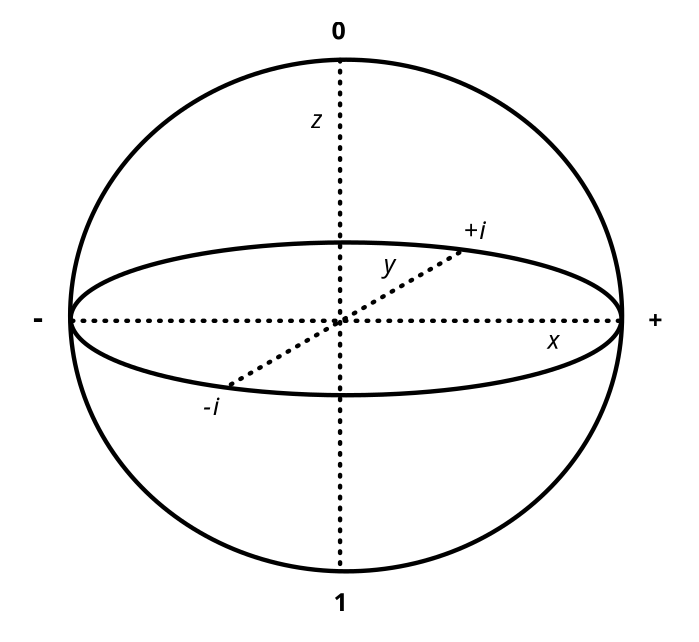
\includegraphics[width=1\linewidth]{Bloch.png}

\end{wrapfigure}
I punti interni rappresentano stati misti, in particolare il centro $\vec{r}=(0,0,0)$ corrisponde allo \textbf{Stato massimalmente misto} $$\rho(\vec{r})=\tau = \frac{\mathbb{1}}{2}$$
Un vettore $\vec{r}=(0,0,2p-1)$ sull'asse $\vec{z}$ con $p\in[0,1]$ corrisponde ad uno stato classico
$$\rho = \frac{1}{2}(\mathbb{1} + (zp-1)Z) = \frac{1}{2}
\begin{pmatrix}
    1+(2p-1) & 0\\
    0 & 1-(2p-1)
\end{pmatrix}
$$
$$
= \begin{pmatrix}
    p & 0\\
    0 & 1-p
\end{pmatrix}
$$
Vediamo quali stati sono intersezione degli assi con la sfera:
\begin{itemize}
    \item Asse $\vec{z}$: \\$\vec{r}=(0,0,1)= \ket{0}$ , $\vec{r}=(0,0,-1)= \ket{1}$
    \item Asse $\vec{x}$: \\$\vec{r}=(1,0,0)= \ket{+}= \frac{1}{\sqrt{2}}(\ket{0} + \ket{1})$ , $\vec{r}=(-1,0,0)= \ket{-}= \frac{1}{\sqrt{2}}(\ket{0} - \ket{1})$
    \item Asse $\vec{y}$: \\$\vec{r}=(0,1,0)= \ket{+i}= \frac{1}{\sqrt{2}}(\ket{0} + i\ket{1})$ , $\vec{r}=(0,-1,0)= \ket{-i}= \frac{1}{\sqrt{2}}(\ket{0} - i\ket{1})$
\end{itemize}

Abbiamo ottenuto 3 diverse basi di $\mathbb{C^2}$, che chiamiamo basi $X,Y,Z$
\begin{itemize}
    \item I vettori della base $X$ sono gli autovettori $\ket{\pm}$ della matrice di Pauli $X$
    \item I vettori della base $Y$ sono gli autovettori $\ket{\pm i}$ della matrice di Pauli $Y$
    \item I vettori della base $Z$ sono gli autovettori $\ket{0},\ket{1}$ della matrice di Pauli $Z$
\end{itemize}

\section{Misurazioni}
Definizione: una \textbf{Misurazione} o \textbf{POVM} (\textit{Positive-Operator-valued-mesure}) su uno spazio di Hilbert con insieme dei risultati $\Omega$ è una collezione di operatori: $\mu=\left\{ \mu(x) \in \textit{PSD}(\mathcal{H}) \right\}_{x\in\Omega}$ t.c $\sum_{x\in\Omega} \mu(x) = \mathbb{1}$.
\medskip
\\Denotiamo con $\textit{meas}(\mathcal{H},\Omega)$ l'insieme di tutte le misure su $\mathcal{H}$ con l'insieme dei risultati in $\Omega$, inoltre $0\le\mu_x\le\mathbb{1}$ dove $\mu_x=\mu(x)$ sono operatori che hanno autovalore $\lambda:0\le\lambda\le1 \hspace{0.3cm} \forall x \in \Omega$
\newpage
\textbf{ASSIOMA 3 (Misurazioni)}
\\Quando eseguiamo una misurazione $\mu\in \textit{Meas}(\mathcal{H},\Omega)$ su uno stato quantistico $\rho\in S(\mathcal{H})$ osserviamo il risultato $x\in \Omega$ con probabilità $$p(x) = \text{tr}[\mu_x\rho]$$
Vediamo un esempio: con un singolo qubit consideriamo $\Omega= \{0,1\}$, e \\$\mu=\{\mu_0,\mu_1\}:\mu_0=\ket{0}\bra{0},\mu_1=\ket{1}\bra{1}$, che definisce una misurazione. Misuriamo $\rho = \ket{\psi}\bra{\psi}$ per $\ket{\psi} = \ket{0}$

$$
    p(0)=\text{tr}[\mu_0\rho]=\text{tr}[\ket{0}\bra{0}\ket{0}\bra{0}] = 1
$$

$$
    p(1)=\text{tr}[\mu_1\rho]=\text{tr}[\ket{1}\bra{1}\ket{0}\bra{0}] = 0
$$

se invece $\ket{\psi} = \ket{+}$

$$
    p(0) = \text{tr}[\ket{0}\bra{0}\frac{1}{2}(\ket{0}+\ket{1})(\ket{0}+\ket{1})] = 
$$
$$
    = \frac{1}{2} \text{tr}\left[
    \begin{pmatrix}
        1 & 0\\
        0 & 0
    \end{pmatrix}
    \begin{pmatrix}
        1 & 1\\
        1 & 1
    \end{pmatrix}
    \right]
     = 
     \frac{1}{2} \text{tr}\left[
    \begin{pmatrix}
        1 & 0\\
        0 & 0
    \end{pmatrix}\right] = \frac{1}{2}
$$

analogamente $p(1) = \frac{1}{2}$.
\\Se consideriamo lo stato massimamente misto $\tau = \frac{1}{2}\mathbb{1}$
$$p(0)=\text{tr}[\ket{0}\bra{0}\frac{1}{2}\mathbb{1}] = \frac{1}{2}$$
e analogamente $p(1) = \frac{1}{2}$, cioè dalla misurazione non sappiamo distinguere $\ket{+}$ da $\tau$
\subsection{Misure rispetto a una base e misure proiettive}
Sia $\left\{\ket{e_x} \right\}_{x\in \Omega}$ una base arbitraria. Allora possiamo costruire una misurazione con l'insieme dei risultati $\Omega$, definendo
$$
    \mu_x = \ket{e_x}\bra{e_x} \hspace{0.3cm}\text{ per } x \in \Omega
$$
Quindi $\sum_{x\in\Omega}\mu_x = \sum_x \ket{e_x}\bra{e_x} = \mathbb{1}$ è una misura valida. Questo tipo di misura si chiama misura rispetto ad una base. In particolare, prendendo la base standard $\left\{ \ket{x} \right\}_{x\in\Sigma}$ otteniamo una misurazione rispetto alla base standard ($\Sigma$ insieme degli stati classici).
\medskip
\\ \textbf{Lemma 3.1} (\textit{Born's rule}): Dato lo stato quantistic $\rho \in S(\mathcal{H})$, eseguendo una misura rispetto ad una base $\mu_x=\ket{e_x}\bra{e_x}$ osserviamo il risultato $x\in\Omega$ con probabilità $p(x)=\braket{e_x|\rho|e_x}$. Inoltre se $\rho = \ket{\psi}\bra{\psi}$ è uno stato puro $\ket{\psi}= \sum_{x\in\Omega}\Psi_x\ket{e_x}$ allora $p(x)=|\Psi_x|^2$
\medskip
\\ \textbf{Dimostrazione:} poichè se $N = \ket{\psi}\bra{\psi}$ abbiamo che  tr$[MN]=\braket{\psi|M|\psi}$, allora $p(x)= \text{tr}[\ket{e_x}\bra{e_x}\rho]=\braket{e_x|\rho|e_x}$. Quando $\rho = \ket{\psi}\bra{\psi}$, $\ket{\psi} = \sum_{x\in\Omega}\Psi_x\ket{\psi}$ otteniamo $p(x)=\braket{e_x|\psi} \braket{\psi|e_x}= |\braket{\psi|e_x}|^2=|\Psi|^2$
\medskip
\\Un caso più generale avviene quando gli operatori di misura $\mu_x$ sono tutte proiezioni, $\mu_x=P_x$. In tal caso abbiamo un operatore di misura proiettiva (\textit{PVM}). $\sum_{x\in\Omega}\mu_x = \mathbb{1}$, le immagini degli $\mu_x$ devono essere ortogonali e spannare tutto.
\subsection{Misurazione di qubit}
In generale scegliamo $\vec{r}=(x,y,z)$ con $||\vec{r}||=1$ e lo stato corrispettivo $-\vec{r}$. Allora 
$$\mu_{\vec{r},0}=p(\vec{r})=\frac{1}{2}
\begin{pmatrix}
    1+z & x-iy\\
    x+iy & 1-z
\end{pmatrix}, 
\mu_{-\vec{r},0}=p(-\vec{r})=\frac{1}{2}
\begin{pmatrix}
    1-z & -x+iy\\
    -x-iy & 1+z
\end{pmatrix}
$$
Se eseguiamo questa nìmisura su uno o stato quantistico con vettore di Bloch $\vec{s}=(x',y',z')$ allora la probabilità di ottenere $0$ è $p(0)= \frac{1}{2}+\frac{1}{2}\vec{r}\cdot\vec{s}=\frac{1}{2}+\frac{1}{2}(xx'+yy'+zz')$. Non esiste alcuno stato quantistico per cui entrambe le misure $X$ e $Z$ sono certe. Le misurazioni mappano uno stato quantistico in uno stato classico.
\medskip
\\ \textbf{Lemma 3.2:} $\Omega$ insieme dei risultati, $\mathcal{H}$ spazio di Hilbert, supponiamo che per ogni $\rho\in S(\mathcal{H})$ esista una distribuzone di probabilità $p\rho\in P(\Omega): p\rho =p_1\rho_1+p_2\rho_2$ perogni stato misto
$\rho = p_1\rho_1+p_2\rho_2$. Allora, esiste un operatore di misura $\mu:\Omega\rightarrow\textit{PSD}(\mathcal{H}):\forall x\in\Omega, p\rho(x)=\textit{tr}[\mu(x)\rho]$

\section{Sistemi quantistici multipli}
Se $\mathcal{H}$ ha una base indicizzata $\ket{x_j}$ da $\ket{x_j}\in \Sigma_j$, allora il prodotto tensoriale $\mathcal{H}_1\otimes\mathcal{H}_2\otimes\dots\otimes\mathcal{H}_n$ ha la base prodotto $\ket{x_1,x_2,\dots,x_n}=\ket{x_1}\ket\otimes{x_2}\otimes\dots\otimes\ket{x_n}$
\medskip
\\ \textbf{ASSIOMA 4 (Sistemi multipli)}
\\Se abbiamo n sistemi quantistici con rispettivi spazi di hilbert $\mathcal{H}_1,\mathcal{H}_2,\dots,\mathcal{H}_n$, allora il sistema congiunto è associato allo spazio di Hilbert $\mathcal{H}_1\otimes\mathcal{H}_2\otimes\dots\otimes\mathcal{H}_n$
\medskip
\\ \textit{Notazione:} $A,B,C $ :Sistemi, $\hspace{0.5cm}\mathcal{H}_A,\mathcal{H}_B,\mathcal{H}_C$ : Spazi associati
\medskip
\\ $\rho_A,\rho_B,\rho_C,\rho_{AB},\rho_{BC},\rho_{AC},\rho_{ABC}$: Stati cogiuti
\medskip
\\$\Sigma_A,\Sigma_B,\Sigma_C$: Alfabeti di simboli
\medskip
\\ $\textit{lin}(A)= \textit{lin}(\mathcal{H}_A)$, $\hspace{0.3cm}S(A) = S(\mathcal{H}_A)$, $\hspace{0.3cm}\textit{PSD}(A)= \textit{PSD}(\mathcal{H}_A)$
\medskip
\\ $\mu_A\in\textit{Meas}(\mathcal{H}_A,\Omega)$, $\hspace{0.5cm}\Sigma_{AB}= \Sigma_A\times\Sigma_B$
\medskip
\\ \textit{Defizione}: $A,B$ stati quabtistici. Gli stati  nella forma $\rho=\rho_A\otimes\rho_B,\rho_A\in S(A),\rho_B\in S(B)$ si chiama \textbf{Stato prodotto}. Uno stato che non è prodotto si dice \textbf{Stato correlato}.
\\Se abbiamo $N$ sistemi, $\rho_{A_1,\dots,A_n}\in S(A_1,\dots,A_n)$ è uno stato prodotto se $\rho_{A_1,\dots,A_n}=\rho_{A_1}\otimes\dots\otimes\rho_{A_n},\hspace{0.3cm}\rho_{A_i}\in S(A_i)$
\medskip
\\ \textbf{Esempio:} $\mathcal{H}_A = \mathcal{H}_b = \mathbb{C}^2 \hspace{0.5cm} \mathcal{H}_A\otimes\mathcal{H}_B \cong
\mathbb{C}^4$
\begin{itemize}
    \item Potrebbero condividere uno degli stati base: $\ket{00},\ket{01},\ket{10},\ket{11}$, stati puri e classici
    \item Potrebbero avere $\ket{+}_A\ket{+}_B= \frac{1}{2}\left( \ket{00}+\ket{01}+\ket{10}+\ket{11} \right)$
    \item Uno stato classico non prodotto si dice \textbf{Massimamente correlato} e corrisponde a 2 bit che sono uguali a 0 o 1.
    $$
        \begin{pmatrix}
            1 &0 &0 &0\\
            0 &0 &0 &0\\
            0 &0 &0 &0\\
            0 &0 &0 &1
        \end{pmatrix}
    $$
    \item  Se abbiamo uno stato non classico e non prodotto si dice \textbf{Massimamente entangled} 
    $$\ket{\Phi^+}_{AB}=\frac{1}{\sqrt{2}}(\ket{00}+\ket{11})  \hspace{0.5cm}  \rho_{AB}=\ket{\Phi^+}_{AB}\bra{\Phi^+}_{AB}$$
    $$=\frac{1}{2}(\ket{00}\bra{00}+\ket{00}\bra{11}+\ket{11}\bra{00}+\ket{11}\bra{11})$$
    $$=
        \begin{pmatrix}
            1 & 0 & 0 & 1 \\
            0 & 0 & 0 & 0 \\
            0 & 0 & 0 & 0 \\
            1 & 0 & 0 & 1
        \end{pmatrix}
    $$
    $$=\frac{1}{2}(\ket{0}\bra{0}\otimes\ket{0}\bra{0}+\ket{0}\bra{1}\otimes\ket{0}\bra{1}+\ket{1}\bra{0}\otimes\ket{1}\bra{0}+\ket{1}\bra{1}\otimes\ket{1}\bra{1})$$
\end{itemize}


\section{Traccia Parziale}
Sia $\mu_A=\{\mu_A(x)\}_{x\in\Omega} \in \textit{Meas}\{A,\Omega\}$ una misurazione che Alice vuole effettuare sul suo sistema.\\
Supponiamo che Alice e Bob condividano uno stato quantistico ma non possano comunicare. Esiste un modo per avere solo lo stato $\rho_A$?
\medskip\\
La maniera più naturale di estendere questa misurazione al sistema $AB$ è considerare la misurazione Globale che esegue 
$\mu_A$ su $A$ e non fa nulla su $B$:

$$
    \mu_A\otimes\mathbb{1}_B=\{\mu_A(x)\otimes\mathbb{1}_B:x\in\Omega\}
$$

È una misurazione valida?
\begin{description}
    \item[i]    $\sum_{x\in\Omega}(\mu_A(x)\otimes\mathbb{1_B})=\left(\sum_{x\in A}\right)\otimes\mathbb{1}_B =\mathbb{1}_A\otimes\mathbb{1}_B=\mathbb{1}_{AB}$
    \item[ii]   $\mu_A(x)\otimes\mathbb{1}_B$ è PSD $\forall x \in \Omega$, il loro prodotto è PSD
\end{description}

In generale se Alice e Bob eseguono $\mu_A$ e $\mu_B$, rispettivamente con insieme dei risultati $\Omega_1$ e $\Omega_2$, corrispondono ad una misurazione sul sistema globale

$$
    \mu_A\otimes\mu_B:=\left\{ \mu_A(x)\otimes\mu_B(y) :(x,y)\in \Omega_1 \times\Omega_2 \right\}
$$

Si osservi che in tal caso, le sole probabilità dei risultati di Alice non dipendono da quelle dei risultati di bob
\medskip\\
Adesso vogliamo ricostruire una descrizione appropriata dello stato di ALice quando il sistema globale si trova nello stato $\rho_{AB}$. Vorremmo che:

\end{document}
